\chapter[Product]{Design and Implementation}
\label{design}

\begin{multicols*}{2}

	\section{Introduction}
		% TODO - Here I will give an overview of the following sections.

	\section{Tools}
		% TODO - This section will cover the various tools I used to complete the product itself, and why I chose them as opposed to any alternatives.

		% Talk about how you decide to use an existing engine you knew well (save time reinventing the wheel for things like lighting, camera stuff, etc)
		% Also you wanted to limit the amount of outside variables as possible, so an existing engine helped with that

	\section{Product model}
		% TODO - This section will contain models of the various states and relations between the functions and other workings of the product, for areas such as the transition between non-Euclidean world areas.
		\autoref{appendix:code:player}

\end{multicols*}

	\begin{figure}[h]
		\label{design:fig:maths}
		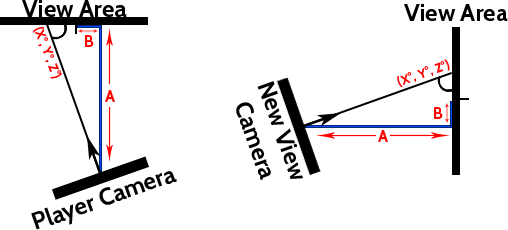
\includegraphics[width=0.8\textwidth]{Images/Position}
		\centering
		\caption{2D representation of the calculations for the position and rotation of cameras.
			See \autoref{appendix:code:camera} for the implementation}
	\end{figure}

	\begin{figure}[h]
		\label{design:fig:scene}
		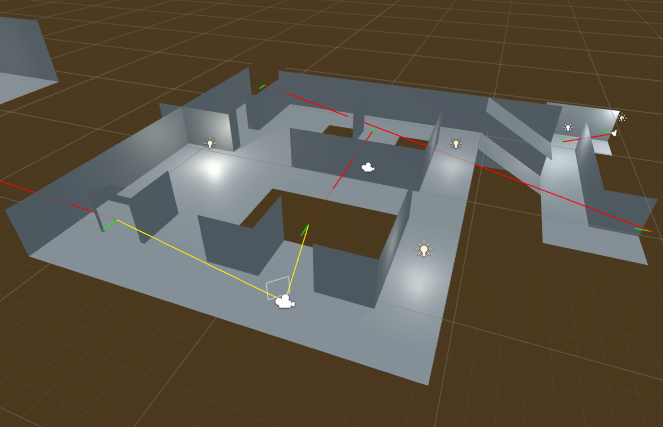
\includegraphics[width=1\textwidth]{Images/Lines_Everywhere2}
		\centering
		\caption{Example view of a scene.
			Red lines are connections between points,
			yellow lines are connections visible to the player,
			and green lines are the direction the connectors are facing}
	\end{figure}

	\begin{figure}[h]
		\label{design:fig:game}
		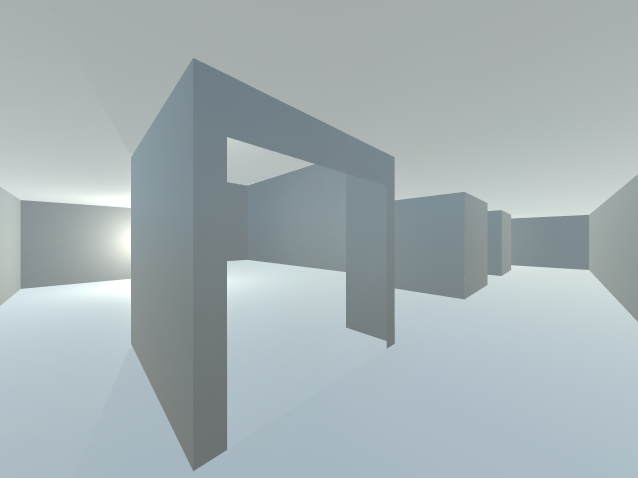
\includegraphics[width=1\textwidth]{Images/NE_View}
		\centering
		\caption{Example of view from inside the Non-Euclidean scene, displaying an area which is larger on the inside}
	\end{figure}

\begin{multicols*}{2}

	\section][Environment Design]{Design of experiment environments}
		% TODO - Here I will be covering the designs of the various areas of the virtual environments to be used in the experiments themselves, and why they are applicable for use for the tests.


\end{multicols*}
